\begin{figure}[H]
    \centering
    \begin{subfigure}[b]{0.4\textwidth}
        \centering
        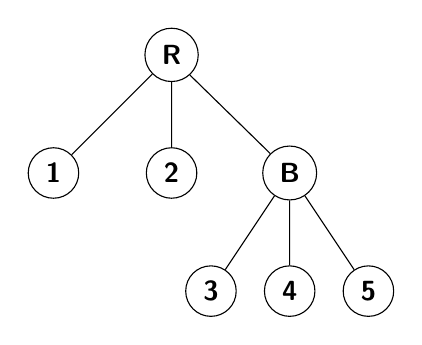
\begin{tikzpicture}[
            level distance=1.5cm,
            level 1/.style={sibling distance=1.5cm},
            level 2/.style={sibling distance=1cm},
            main node/.style={circle,draw,font=\sffamily\bfseries}]
                    % Define vertices
            \node[main node] (R) {R}
            child {node[main node] (1) {1}}
            child {node[main node] (2) {2}}
            child {node[main node] (B) {B}
                child {node[main node] (3) {3}}
                child {node[main node] (4) {4}}
                child {node[main node] (5) {5}}
            };
        \end{tikzpicture}
        \label{fig:example_scc_tree}
    \end{subfigure}
    \hfill
    \begin{subfigure}[b]{0.25\textwidth}
        \centering
        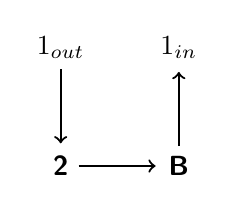
\begin{tikzpicture}[
            ->,shorten >=1pt,auto,node distance=1.5cm,
            thick,main node/.style={font=\sffamily\bfseries}]
            % Define vertices
        \node[main node] (1) {$1_{in}$};
        \node[main node] (11) [left of=1] {$1_{out}$};
        \node[main node] (2) [below of=11] {2};
        \node[main node] (B) [below of=1] {B};
        

        % Draw edges
        \path[every node/.style={font=\sffamily\small}]
            (11) edge (2)
            (2) edge (B)
            (B) edge (1);
        \end{tikzpicture}
        \caption{STN(R)}
        \label{fig:stn_r}
    \end{subfigure}
    \hfill 
    \begin{subfigure}[b]{0.25\textwidth}
        \centering
        \begin{tikzpicture}[
            ->,shorten >=1pt,auto,node distance=1.5cm,
            thick,main node/.style={font=\sffamily\bfseries}]
            % Define vertices
        \node[main node] (3) {$3_{in}$};
        \node[main node] (33) [left of=1] {$3_{out}$};
        \node[main node] (4) [below of=11] {4};
        \node[main node] (5) [below of=1] {5};
        

        % Draw edges
        \path[every node/.style={font=\sffamily\small}]
            (33) edge (4)
            (4) edge (5)
            (5) edge (3);
        \end{tikzpicture}
        \caption{STN(B)}
        \label{fig:stn_b}
    \end{subfigure}
    \caption{Example SCC Tree and its corresponding STNs}
    \label{fig:figure_with_subfigures}
\end{figure}

The SCC tree shown in \figureref{\ref{fig:figure_with_subfigures}}, can be represented by a collection of STNs as follows:
\begin{itemize}
    \item $\text{\textit{STN}}(R)=(\{1,2,B\}, \{(1,2), (2,B), (B,1)\})$
    \item $\text{\textit{STN}}(B)=(\{3,4,5\}, \{(3,4), (4,5), (5,3)\})$
    \item $\text{\textit{STN}}(v)=\lf(\{v\}, \emptyset\rt) \forall v \in \{1,2,3,4,5\}$
\end{itemize}
The SCC tree represented by label $B$ contains the STNs of $\{B,3,4,5\}$, which form a subtree of the SCC tree represented by label $R$,
similarly, the SCC tree represented by labels $\{1,2\}$ also form $R$'s subtree.